\documentclass[twoside]{book}

% Packages required by doxygen
\usepackage{fixltx2e}
\usepackage{calc}
\usepackage{doxygen}
\usepackage[export]{adjustbox} % also loads graphicx
\usepackage{graphicx}
\usepackage[utf8]{inputenc}
\usepackage{makeidx}
\usepackage{multicol}
\usepackage{multirow}
\PassOptionsToPackage{warn}{textcomp}
\usepackage{textcomp}
\usepackage[nointegrals]{wasysym}
\usepackage[table]{xcolor}

% Font selection
\usepackage[T1]{fontenc}
\usepackage[scaled=.90]{helvet}
\usepackage{courier}
\usepackage{amssymb}
\usepackage{sectsty}
\renewcommand{\familydefault}{\sfdefault}
\allsectionsfont{%
  \fontseries{bc}\selectfont%
  \color{darkgray}%
}
\renewcommand{\DoxyLabelFont}{%
  \fontseries{bc}\selectfont%
  \color{darkgray}%
}
\newcommand{\+}{\discretionary{\mbox{\scriptsize$\hookleftarrow$}}{}{}}

% Page & text layout
\usepackage{geometry}
\geometry{%
  a4paper,%
  top=2.5cm,%
  bottom=2.5cm,%
  left=2.5cm,%
  right=2.5cm%
}
\tolerance=750
\hfuzz=15pt
\hbadness=750
\setlength{\emergencystretch}{15pt}
\setlength{\parindent}{0cm}
\setlength{\parskip}{3ex plus 2ex minus 2ex}
\makeatletter
\renewcommand{\paragraph}{%
  \@startsection{paragraph}{4}{0ex}{-1.0ex}{1.0ex}{%
    \normalfont\normalsize\bfseries\SS@parafont%
  }%
}
\renewcommand{\subparagraph}{%
  \@startsection{subparagraph}{5}{0ex}{-1.0ex}{1.0ex}{%
    \normalfont\normalsize\bfseries\SS@subparafont%
  }%
}
\makeatother

% Headers & footers
\usepackage{fancyhdr}
\pagestyle{fancyplain}
\fancyhead[LE]{\fancyplain{}{\bfseries\thepage}}
\fancyhead[CE]{\fancyplain{}{}}
\fancyhead[RE]{\fancyplain{}{\bfseries\leftmark}}
\fancyhead[LO]{\fancyplain{}{\bfseries\rightmark}}
\fancyhead[CO]{\fancyplain{}{}}
\fancyhead[RO]{\fancyplain{}{\bfseries\thepage}}
\fancyfoot[LE]{\fancyplain{}{}}
\fancyfoot[CE]{\fancyplain{}{}}
\fancyfoot[RE]{\fancyplain{}{\bfseries\scriptsize Generated by Doxygen }}
\fancyfoot[LO]{\fancyplain{}{\bfseries\scriptsize Generated by Doxygen }}
\fancyfoot[CO]{\fancyplain{}{}}
\fancyfoot[RO]{\fancyplain{}{}}
\renewcommand{\footrulewidth}{0.4pt}
\renewcommand{\chaptermark}[1]{%
  \markboth{#1}{}%
}
\renewcommand{\sectionmark}[1]{%
  \markright{\thesection\ #1}%
}

% Indices & bibliography
\usepackage{natbib}
\usepackage[titles]{tocloft}
\setcounter{tocdepth}{3}
\setcounter{secnumdepth}{5}
\makeindex

% Hyperlinks (required, but should be loaded last)
\usepackage{ifpdf}
\ifpdf
  \usepackage[pdftex,pagebackref=true]{hyperref}
\else
  \usepackage[ps2pdf,pagebackref=true]{hyperref}
\fi
\hypersetup{%
  colorlinks=true,%
  linkcolor=blue,%
  citecolor=blue,%
  unicode%
}

% Custom commands
\newcommand{\clearemptydoublepage}{%
  \newpage{\pagestyle{empty}\cleardoublepage}%
}

\usepackage{caption}
\captionsetup{labelsep=space,justification=centering,font={bf},singlelinecheck=off,skip=4pt,position=top}

%===== C O N T E N T S =====

\begin{document}

% Titlepage & ToC
\hypersetup{pageanchor=false,
             bookmarksnumbered=true,
             pdfencoding=unicode
            }
\pagenumbering{alph}
\begin{titlepage}
\vspace*{7cm}
\begin{center}%
{\Large My Project }\\
\vspace*{1cm}
{\large Generated by Doxygen 1.8.13}\\
\end{center}
\end{titlepage}
\clearemptydoublepage
\pagenumbering{roman}
\tableofcontents
\clearemptydoublepage
\pagenumbering{arabic}
\hypersetup{pageanchor=true}

%--- Begin generated contents ---
\chapter{Short Description of the Program}
\label{index}\hypertarget{index}{}\begin{DoxyAuthor}{Author}
Tristan Karch
\end{DoxyAuthor}
This program uses a restrictive algorithm to compute the F\+FT of an image and to perfrom basic operation of image processing based on the Fourier domain. The program is linked and built using the cmake method. In order to be able to use it, the user must have installed the magick++ library from the Image\+Magick A\+PI. The Cmake\+List.\+txt file is provided with all the source file. The user is invited to comment or uncomment the lines corresponding to the OS on which he is using the program.

All kind of image can be read. If they are in R\+GB format, they are automatically converted to grayscale. The gray levels are defined to start from 0 and go to 255, 0 being black and 255 being white.

Three different types of padding are implemented \+:
\begin{DoxyItemize}
\item Mirror Folding
\item Zero Padding
\item Periodization
\end{DoxyItemize}

Two types of filters are implemented \+:
\begin{DoxyItemize}
\item Noise removing (Low Pass Filter)
\item Edge Detection (High Pass Filter)
\end{DoxyItemize}

Restriction \+:
\begin{DoxyItemize}
\item Only grayscale images are treated
\item The input images can only be of size that are multiple of two
\item The padding is always extending the size of the image by two
\item The filters implemented are always centered at the origin. Hence no band cut or band pass can be performed
\end{DoxyItemize}

The user has the following choice when running the main \+:
\begin{DoxyItemize}
\item The name of the input image on which the operations are going to be carried out.
\item The type of Padding desired
\item The type of Filtering desired
\item The gain of the filter (must be between 0 and 1)
\end{DoxyItemize}

The default output are \+:
\begin{DoxyItemize}
\item The histogram (contained in the file histogram.\+dat)
\item The filtered image in the file named as desired
\item The Phase and Magnitude of the image after and before filtering (contained in the files magnitude/phase\+\_\+filtered.\+png and magnitude/phase\+\_\+origin.\+png)
\end{DoxyItemize}

Note to the professor \+: I have built my project on my mac and everything is compiling fine with cmake. I hope that the note that I have put in the C\+Make\+Lists.\+txt also work on the Linux platform. 
\chapter{Hierarchical Index}
\section{Class Hierarchy}
This inheritance list is sorted roughly, but not completely, alphabetically\+:\begin{DoxyCompactList}
\item \contentsline{section}{Abstract\+Padding}{\pageref{class_abstract_padding}}{}
\begin{DoxyCompactList}
\item \contentsline{section}{Mirror\+Padding}{\pageref{class_mirror_padding}}{}
\item \contentsline{section}{Periodization\+Padding}{\pageref{class_periodization_padding}}{}
\item \contentsline{section}{Unpad}{\pageref{class_unpad}}{}
\item \contentsline{section}{Zero\+Padding}{\pageref{class_zero_padding}}{}
\end{DoxyCompactList}
\item \contentsline{section}{Complex\+Number}{\pageref{class_complex_number}}{}
\item \contentsline{section}{F\+F\+T\+Pix}{\pageref{class_f_f_t_pix}}{}
\item \contentsline{section}{Image\+Pix$<$ pixel $>$}{\pageref{class_image_pix}}{}
\item \contentsline{section}{Image\+Pix$<$ Complex\+Number $>$}{\pageref{class_image_pix}}{}
\item \contentsline{section}{Image\+Pix$<$ int $>$}{\pageref{class_image_pix}}{}
\end{DoxyCompactList}

\chapter{Class Index}
\section{Class List}
Here are the classes, structs, unions and interfaces with brief descriptions\+:\begin{DoxyCompactList}
\item\contentsline{section}{\hyperlink{class_abstract_padding}{Abstract\+Padding} }{\pageref{class_abstract_padding}}{}
\item\contentsline{section}{\hyperlink{class_complex_number}{Complex\+Number} }{\pageref{class_complex_number}}{}
\item\contentsline{section}{\hyperlink{class_f_f_t_pix}{F\+F\+T\+Pix} }{\pageref{class_f_f_t_pix}}{}
\item\contentsline{section}{\hyperlink{class_image_pix}{Image\+Pix$<$ pixel $>$} }{\pageref{class_image_pix}}{}
\item\contentsline{section}{\hyperlink{class_mirror_padding}{Mirror\+Padding} }{\pageref{class_mirror_padding}}{}
\item\contentsline{section}{\hyperlink{class_periodization_padding}{Periodization\+Padding} }{\pageref{class_periodization_padding}}{}
\item\contentsline{section}{\hyperlink{class_unpad}{Unpad} }{\pageref{class_unpad}}{}
\item\contentsline{section}{\hyperlink{class_zero_padding}{Zero\+Padding} }{\pageref{class_zero_padding}}{}
\end{DoxyCompactList}

\chapter{Class Documentation}
\hypertarget{class_abstract_padding}{}\section{Abstract\+Padding Class Reference}
\label{class_abstract_padding}\index{Abstract\+Padding@{Abstract\+Padding}}


{\ttfamily \#include $<$Abstract\+Padding.\+hpp$>$}

Inheritance diagram for Abstract\+Padding\+:\begin{figure}[H]
\begin{center}
\leavevmode
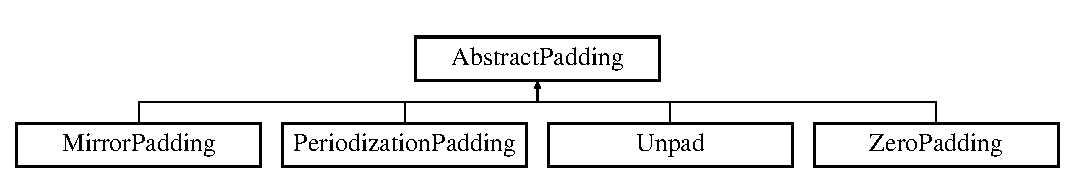
\includegraphics[height=2.000000cm]{class_abstract_padding}
\end{center}
\end{figure}
\subsection*{Public Member Functions}
\begin{DoxyCompactItemize}
\item 
\mbox{\Hypertarget{class_abstract_padding_a1718652cce1bfac03d7e3918b5d380bd}\label{class_abstract_padding_a1718652cce1bfac03d7e3918b5d380bd}} 
virtual \hyperlink{class_image_pix}{Image\+Pix}$<$ int $>$ {\bfseries Perform\+Pad} (\hyperlink{class_image_pix}{Image\+Pix}$<$ int $>$ \&in)=0
\end{DoxyCompactItemize}


\subsection{Detailed Description}
Abstract class to perform different kind of padding and also to perform the unpading operation. The width and height of the images are allways extended by two so that the 2raddix fft algorithm can still be performed once the image is padded. 

The documentation for this class was generated from the following files\+:\begin{DoxyCompactItemize}
\item 
Abstract\+Padding.\+hpp\item 
Abstract\+Padding.\+cpp\end{DoxyCompactItemize}

\hypertarget{class_complex_number}{}\section{Complex\+Number Class Reference}
\label{class_complex_number}\index{Complex\+Number@{Complex\+Number}}


{\ttfamily \#include $<$Complex\+Number.\+hpp$>$}

\subsection*{Public Member Functions}
\begin{DoxyCompactItemize}
\item 
\mbox{\Hypertarget{class_complex_number_a2226acaab891160ba96a93249f624ae8}\label{class_complex_number_a2226acaab891160ba96a93249f624ae8}} 
{\bfseries Complex\+Number} (double x, double y)
\item 
\mbox{\Hypertarget{class_complex_number_a39b29f461cfdec50516415054e583907}\label{class_complex_number_a39b29f461cfdec50516415054e583907}} 
{\bfseries Complex\+Number} (const \hyperlink{class_complex_number}{Complex\+Number} \&c)
\item 
\mbox{\Hypertarget{class_complex_number_af09f875c9fe74b4e037fe0c112f87021}\label{class_complex_number_af09f875c9fe74b4e037fe0c112f87021}} 
{\bfseries Complex\+Number} (const double d)
\item 
\mbox{\Hypertarget{class_complex_number_a06a85cd26304575eb711b758de7ed48c}\label{class_complex_number_a06a85cd26304575eb711b758de7ed48c}} 
double {\bfseries Get\+Real\+Part} () const
\item 
\mbox{\Hypertarget{class_complex_number_abc6aa475c80076146c0b3694be4c6d1a}\label{class_complex_number_abc6aa475c80076146c0b3694be4c6d1a}} 
double {\bfseries Get\+Imaginary\+Part} () const
\item 
\mbox{\Hypertarget{class_complex_number_a81652b57d845e3563edd86fce526704e}\label{class_complex_number_a81652b57d845e3563edd86fce526704e}} 
double {\bfseries Calculate\+Magnitude} () const
\item 
\mbox{\Hypertarget{class_complex_number_a4bc3501f6b8f3a55c9bc7a560095b0ff}\label{class_complex_number_a4bc3501f6b8f3a55c9bc7a560095b0ff}} 
double {\bfseries Calculate\+Argument} () const
\item 
\mbox{\Hypertarget{class_complex_number_a9f6d9f39c74e0f2487a940dd6d15f0a8}\label{class_complex_number_a9f6d9f39c74e0f2487a940dd6d15f0a8}} 
\hyperlink{class_complex_number}{Complex\+Number} {\bfseries Calculate\+Power} (double n) const
\item 
\mbox{\Hypertarget{class_complex_number_a0e5a8c423e3d7381224cec7841ea56cb}\label{class_complex_number_a0e5a8c423e3d7381224cec7841ea56cb}} 
\hyperlink{class_complex_number}{Complex\+Number} {\bfseries Calculate\+Conjugate} () const
\item 
\mbox{\Hypertarget{class_complex_number_affd8dbb8111caffd73bf70e35d8098f5}\label{class_complex_number_affd8dbb8111caffd73bf70e35d8098f5}} 
void {\bfseries Set\+Conjugate} ()
\item 
\mbox{\Hypertarget{class_complex_number_a4e566cd69db5bac44f2ffb3382ebb5e1}\label{class_complex_number_a4e566cd69db5bac44f2ffb3382ebb5e1}} 
\hyperlink{class_complex_number}{Complex\+Number} {\bfseries Complex\+From\+Polar} (double r, double theta\+\_\+radians)
\item 
\mbox{\Hypertarget{class_complex_number_a4f1af0a28c9ad06a27ceb77a4fc115f5}\label{class_complex_number_a4f1af0a28c9ad06a27ceb77a4fc115f5}} 
\hyperlink{class_complex_number}{Complex\+Number} \& {\bfseries operator=} (const \hyperlink{class_complex_number}{Complex\+Number} \&z)
\item 
\mbox{\Hypertarget{class_complex_number_a647004355a5f7f43e6764aa9751615de}\label{class_complex_number_a647004355a5f7f43e6764aa9751615de}} 
\hyperlink{class_complex_number}{Complex\+Number} {\bfseries operator-\/} () const
\item 
\mbox{\Hypertarget{class_complex_number_adf755ed1c8e82c64223c569cd3a744a8}\label{class_complex_number_adf755ed1c8e82c64223c569cd3a744a8}} 
\hyperlink{class_complex_number}{Complex\+Number} {\bfseries operator+} (const \hyperlink{class_complex_number}{Complex\+Number} \&z) const
\item 
\mbox{\Hypertarget{class_complex_number_a62fac8ef31e8f7cf473a4e025216c1f0}\label{class_complex_number_a62fac8ef31e8f7cf473a4e025216c1f0}} 
\hyperlink{class_complex_number}{Complex\+Number} {\bfseries operator-\/} (const \hyperlink{class_complex_number}{Complex\+Number} \&z) const
\item 
\mbox{\Hypertarget{class_complex_number_a7860e52995e602941719801ecca2dcb7}\label{class_complex_number_a7860e52995e602941719801ecca2dcb7}} 
\hyperlink{class_complex_number}{Complex\+Number} {\bfseries operator$\ast$} (const double d) const
\item 
\mbox{\Hypertarget{class_complex_number_a65b84287dd76949b4236adc928a80919}\label{class_complex_number_a65b84287dd76949b4236adc928a80919}} 
\hyperlink{class_complex_number}{Complex\+Number} {\bfseries operator/} (const double d) const
\item 
\mbox{\Hypertarget{class_complex_number_a7134536ba0e91c67c98c91fa3e46ac1f}\label{class_complex_number_a7134536ba0e91c67c98c91fa3e46ac1f}} 
\hyperlink{class_complex_number}{Complex\+Number} {\bfseries operator$\ast$} (const \hyperlink{class_complex_number}{Complex\+Number} \&z) const
\item 
\mbox{\Hypertarget{class_complex_number_ad5286e63745428e443f20a3fe4c41dc6}\label{class_complex_number_ad5286e63745428e443f20a3fe4c41dc6}} 
bool {\bfseries operator$>$} (const \hyperlink{class_complex_number}{Complex\+Number} \&z) const
\item 
\mbox{\Hypertarget{class_complex_number_a109c83599836c2590a722ef632ee6918}\label{class_complex_number_a109c83599836c2590a722ef632ee6918}} 
bool {\bfseries operator$<$} (const \hyperlink{class_complex_number}{Complex\+Number} \&z) const
\end{DoxyCompactItemize}
\subsection*{Friends}
\begin{DoxyCompactItemize}
\item 
\mbox{\Hypertarget{class_complex_number_a8c7adda75cab62a2d6d3a9ec73fa420e}\label{class_complex_number_a8c7adda75cab62a2d6d3a9ec73fa420e}} 
std\+::ostream \& {\bfseries operator$<$$<$} (std\+::ostream \&output, const \hyperlink{class_complex_number}{Complex\+Number} \&z)
\item 
\mbox{\Hypertarget{class_complex_number_a3535de0d1bdf6a1b107d1a39b233cc88}\label{class_complex_number_a3535de0d1bdf6a1b107d1a39b233cc88}} 
double {\bfseries Real\+Part} (const \hyperlink{class_complex_number}{Complex\+Number} \&z)
\item 
\mbox{\Hypertarget{class_complex_number_a97cb10a13c288a75e3830acbcc52028d}\label{class_complex_number_a97cb10a13c288a75e3830acbcc52028d}} 
double {\bfseries Imaginary\+Part} (const \hyperlink{class_complex_number}{Complex\+Number} \&z)
\end{DoxyCompactItemize}


\subsection{Detailed Description}
The class \hyperlink{class_complex_number}{Complex\+Number} contains two private members the real part and the imaginary part of the complex number. It contains the basic algebra to perform all the operations desired for this project 

The documentation for this class was generated from the following files\+:\begin{DoxyCompactItemize}
\item 
Complex\+Number.\+hpp\item 
Complex\+Number.\+cpp\end{DoxyCompactItemize}

\hypertarget{class_f_f_t_pix}{}\section{F\+F\+T\+Pix Class Reference}
\label{class_f_f_t_pix}\index{F\+F\+T\+Pix@{F\+F\+T\+Pix}}


{\ttfamily \#include $<$F\+F\+T\+Pix.\+hpp$>$}

\subsection*{Public Member Functions}
\begin{DoxyCompactItemize}
\item 
\mbox{\Hypertarget{class_f_f_t_pix_a3a2315d33b0012b47af83f1f61da1f2a}\label{class_f_f_t_pix_a3a2315d33b0012b47af83f1f61da1f2a}} 
{\bfseries F\+F\+T\+Pix} (\hyperlink{class_image_pix}{Image\+Pix}$<$ int $>$ \&in, std\+::string)
\item 
\mbox{\Hypertarget{class_f_f_t_pix_a978e768e54677662ec082870e1ce7fa2}\label{class_f_f_t_pix_a978e768e54677662ec082870e1ce7fa2}} 
{\bfseries F\+F\+T\+Pix} (\hyperlink{class_image_pix}{Image\+Pix}$<$ \hyperlink{class_complex_number}{Complex\+Number} $>$ \&in)
\item 
\hyperlink{class_complex_number}{Complex\+Number} $\ast$ \hyperlink{class_f_f_t_pix_aa0b0b6a2bff47b800d3e61770a187ba6}{F\+FT} (\hyperlink{class_complex_number}{Complex\+Number} $\ast$x, int N, bool inverse=false)
\item 
\mbox{\Hypertarget{class_f_f_t_pix_ab28ee558de51f9951106710bf48a9e2f}\label{class_f_f_t_pix_ab28ee558de51f9951106710bf48a9e2f}} 
\hyperlink{class_complex_number}{Complex\+Number} $\ast$ {\bfseries i\+F\+FT} (\hyperlink{class_complex_number}{Complex\+Number} $\ast$x, int N)
\item 
\mbox{\Hypertarget{class_f_f_t_pix_a12fc448d7b8f8dc731621a457da0241a}\label{class_f_f_t_pix_a12fc448d7b8f8dc731621a457da0241a}} 
\hyperlink{class_image_pix}{Image\+Pix}$<$ \hyperlink{class_complex_number}{Complex\+Number} $>$ {\bfseries F\+F\+T2} (\hyperlink{class_image_pix}{Image\+Pix}$<$ \hyperlink{class_complex_number}{Complex\+Number} $>$ \&in)
\item 
\mbox{\Hypertarget{class_f_f_t_pix_acc27a8bd3ee42fba90e30765287822e9}\label{class_f_f_t_pix_acc27a8bd3ee42fba90e30765287822e9}} 
\hyperlink{class_image_pix}{Image\+Pix}$<$ \hyperlink{class_complex_number}{Complex\+Number} $>$ {\bfseries i\+F\+F\+T2} (\hyperlink{class_image_pix}{Image\+Pix}$<$ \hyperlink{class_complex_number}{Complex\+Number} $>$ \&in)
\item 
\mbox{\Hypertarget{class_f_f_t_pix_a15fa556b7d65a6c8e21e451d2184fcd0}\label{class_f_f_t_pix_a15fa556b7d65a6c8e21e451d2184fcd0}} 
\hyperlink{class_image_pix}{Image\+Pix}$<$ int $>$ {\bfseries get\+Space} ()
\item 
\mbox{\Hypertarget{class_f_f_t_pix_ae88f60d77bb4f21eb9a9d7cb68b518a8}\label{class_f_f_t_pix_ae88f60d77bb4f21eb9a9d7cb68b518a8}} 
\hyperlink{class_image_pix}{Image\+Pix}$<$ \hyperlink{class_complex_number}{Complex\+Number} $>$ {\bfseries get\+Fourier} ()
\end{DoxyCompactItemize}


\subsection{Detailed Description}
Class that contains two private members \+:
\begin{DoxyItemize}
\item mspace\+\_\+image is a pointer on the object Image\+Pix$<$int$>$.\+It contains the information of the image in the space domain
\item mfourier\+\_\+image is a pointer on the object \hyperlink{class_image_pix}{Image\+Pix$<$\+Complex\+Number$>$}. It contains the information of the image in the Fourier domain
\end{DoxyItemize}

The constructor computes directly the fourier transform and the inverse fourier transform depending on the input arguments. The methods are only used to compute the F\+FT and the inverse F\+FT and to access the different object pointed by both pointers. 

\subsection{Member Function Documentation}
\mbox{\Hypertarget{class_f_f_t_pix_aa0b0b6a2bff47b800d3e61770a187ba6}\label{class_f_f_t_pix_aa0b0b6a2bff47b800d3e61770a187ba6}} 
\index{F\+F\+T\+Pix@{F\+F\+T\+Pix}!F\+FT@{F\+FT}}
\index{F\+FT@{F\+FT}!F\+F\+T\+Pix@{F\+F\+T\+Pix}}
\subsubsection{\texorpdfstring{F\+F\+T()}{FFT()}}
{\footnotesize\ttfamily \hyperlink{class_complex_number}{Complex\+Number} $\ast$ F\+F\+T\+Pix\+::\+F\+FT (\begin{DoxyParamCaption}\item[{\hyperlink{class_complex_number}{Complex\+Number} $\ast$}]{x,  }\item[{int}]{N,  }\item[{bool}]{inverse = {\ttfamily false} }\end{DoxyParamCaption})}


\begin{DoxyParams}{Parameters}
{\em the} & bool parameter here is only used for the implementation of the inverse F\+FT. It should not be modified by the user. \\
\hline
\end{DoxyParams}


The documentation for this class was generated from the following files\+:\begin{DoxyCompactItemize}
\item 
F\+F\+T\+Pix.\+hpp\item 
F\+F\+T\+Pix.\+cpp\end{DoxyCompactItemize}

\hypertarget{class_image_pix}{}\section{Image\+Pix$<$ pixel $>$ Class Template Reference}
\label{class_image_pix}\index{Image\+Pix$<$ pixel $>$@{Image\+Pix$<$ pixel $>$}}


{\ttfamily \#include $<$Image\+Pix.\+hpp$>$}

\subsection*{Public Member Functions}
\begin{DoxyCompactItemize}
\item 
\mbox{\Hypertarget{class_image_pix_a17f15a447ea6c728e78be078dbc39c50}\label{class_image_pix_a17f15a447ea6c728e78be078dbc39c50}} 
{\bfseries Image\+Pix} (int Nx, int Ny)
\item 
\mbox{\Hypertarget{class_image_pix_a0f23257cc21d600b6b2416fc91a26eb2}\label{class_image_pix_a0f23257cc21d600b6b2416fc91a26eb2}} 
{\bfseries Image\+Pix} (int Pixel\+Array\mbox{[}$\,$\mbox{]}, int width, int height)
\item 
\mbox{\Hypertarget{class_image_pix_ab8c59910169f25c2a8e2636a020383cf}\label{class_image_pix_ab8c59910169f25c2a8e2636a020383cf}} 
int {\bfseries get\+Nx} () const
\item 
\mbox{\Hypertarget{class_image_pix_a14889774c915f6e33d1338441ed90c59}\label{class_image_pix_a14889774c915f6e33d1338441ed90c59}} 
int {\bfseries get\+Ny} () const
\item 
\mbox{\Hypertarget{class_image_pix_a358e87a17ee723b335f03eebfa79a070}\label{class_image_pix_a358e87a17ee723b335f03eebfa79a070}} 
pixel $\ast$ {\bfseries get\+Row} (int x)
\item 
\mbox{\Hypertarget{class_image_pix_a3f90c5b98fe6336fddd09be724dc1c2e}\label{class_image_pix_a3f90c5b98fe6336fddd09be724dc1c2e}} 
pixel $\ast$ {\bfseries get\+Column} (int y)
\item 
\mbox{\Hypertarget{class_image_pix_a96e1577e600cc1cd0733d7785ffb030a}\label{class_image_pix_a96e1577e600cc1cd0733d7785ffb030a}} 
pixel {\bfseries get\+Pixel} (int x, int y) const
\item 
\mbox{\Hypertarget{class_image_pix_a866b265addb010f1c4ec9d377521ba84}\label{class_image_pix_a866b265addb010f1c4ec9d377521ba84}} 
pixel {\bfseries get\+Max} ()
\item 
\mbox{\Hypertarget{class_image_pix_a41fc615e80bb4d560dde39be2f9fb839}\label{class_image_pix_a41fc615e80bb4d560dde39be2f9fb839}} 
pixel {\bfseries get\+Min} ()
\item 
\mbox{\Hypertarget{class_image_pix_a640b8600e6184695c536555c40535f05}\label{class_image_pix_a640b8600e6184695c536555c40535f05}} 
void {\bfseries Set\+Row} (pixel $\ast$row, int x)
\item 
\mbox{\Hypertarget{class_image_pix_a93d91ee1aa9da87ea1cb4b0b302fe5d2}\label{class_image_pix_a93d91ee1aa9da87ea1cb4b0b302fe5d2}} 
void {\bfseries Set\+Column} (pixel $\ast$column, int y)
\item 
\mbox{\Hypertarget{class_image_pix_a34ec822d24acb1899470251f515f703c}\label{class_image_pix_a34ec822d24acb1899470251f515f703c}} 
pixel \& {\bfseries operator()} (int i, int j)
\item 
\mbox{\Hypertarget{class_image_pix_a222c1bf56e0f14be03094c9eb81b6fc1}\label{class_image_pix_a222c1bf56e0f14be03094c9eb81b6fc1}} 
\hyperlink{class_image_pix}{Image\+Pix} \& {\bfseries operator=} (const \hyperlink{class_image_pix}{Image\+Pix} \&im)
\end{DoxyCompactItemize}


\subsection{Detailed Description}
\subsubsection*{template$<$typename pixel$>$\newline
class Image\+Pix$<$ pixel $>$}

Templated class to implement an image either of int or of \hyperlink{class_complex_number}{Complex\+Number} in the Fourrier domain It contains several constructor\+:
\begin{DoxyItemize}
\item a default constructor
\item an empty constructor of the desired size
\item a constructor from the Pixelarray generated while reading an image (see the Image\+Tools.\+cpp file to know how images are read) 
\end{DoxyItemize}

The documentation for this class was generated from the following file\+:\begin{DoxyCompactItemize}
\item 
Image\+Pix.\+hpp\end{DoxyCompactItemize}

\hypertarget{class_mirror_padding}{}\section{Mirror\+Padding Class Reference}
\label{class_mirror_padding}\index{Mirror\+Padding@{Mirror\+Padding}}


{\ttfamily \#include $<$Mirror\+Padding.\+hpp$>$}

Inheritance diagram for Mirror\+Padding\+:\begin{figure}[H]
\begin{center}
\leavevmode
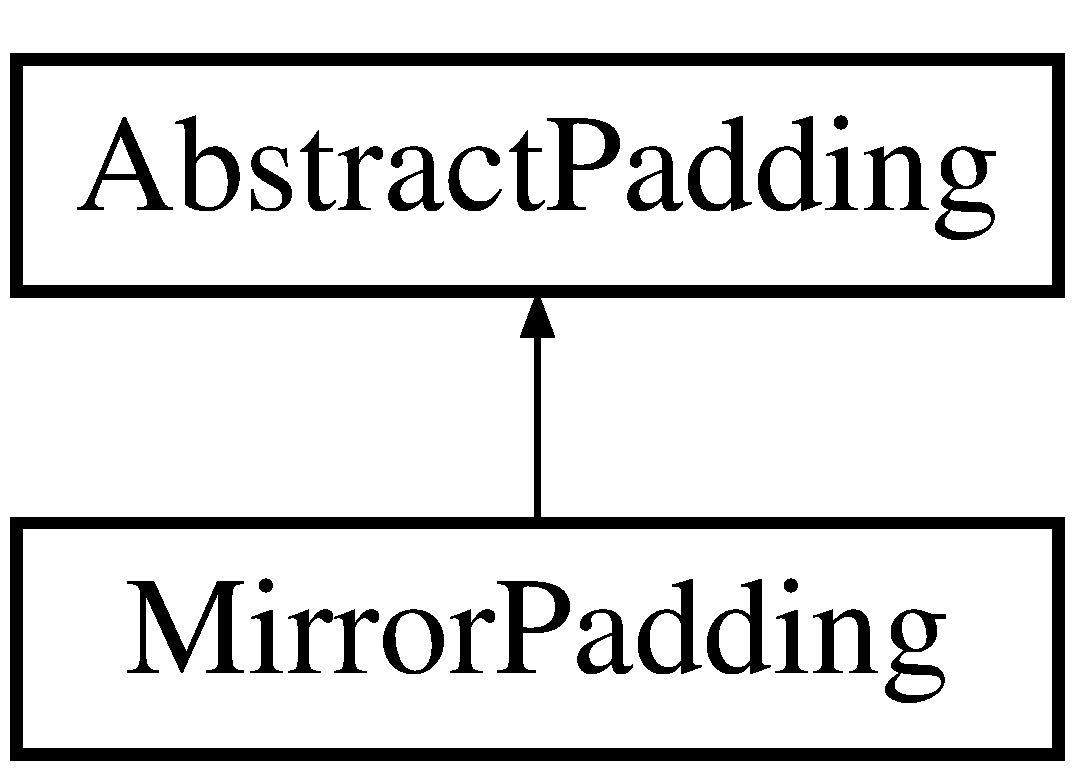
\includegraphics[height=2.000000cm]{class_mirror_padding}
\end{center}
\end{figure}
\subsection*{Public Member Functions}
\begin{DoxyCompactItemize}
\item 
\mbox{\Hypertarget{class_mirror_padding_a61f965646b19bc7efe88ddf2e3825a75}\label{class_mirror_padding_a61f965646b19bc7efe88ddf2e3825a75}} 
\hyperlink{class_image_pix}{Image\+Pix}$<$ int $>$ {\bfseries Perform\+Pad} (\hyperlink{class_image_pix}{Image\+Pix}$<$ int $>$ \&in)
\end{DoxyCompactItemize}


\subsection{Detailed Description}
Performs the Mirror folding of the image. 

The documentation for this class was generated from the following files\+:\begin{DoxyCompactItemize}
\item 
Mirror\+Padding.\+hpp\item 
Mirror\+Padding.\+cpp\end{DoxyCompactItemize}

\hypertarget{class_periodization_padding}{}\section{Periodization\+Padding Class Reference}
\label{class_periodization_padding}\index{Periodization\+Padding@{Periodization\+Padding}}


{\ttfamily \#include $<$Periodization\+Padding.\+hpp$>$}

Inheritance diagram for Periodization\+Padding\+:\begin{figure}[H]
\begin{center}
\leavevmode
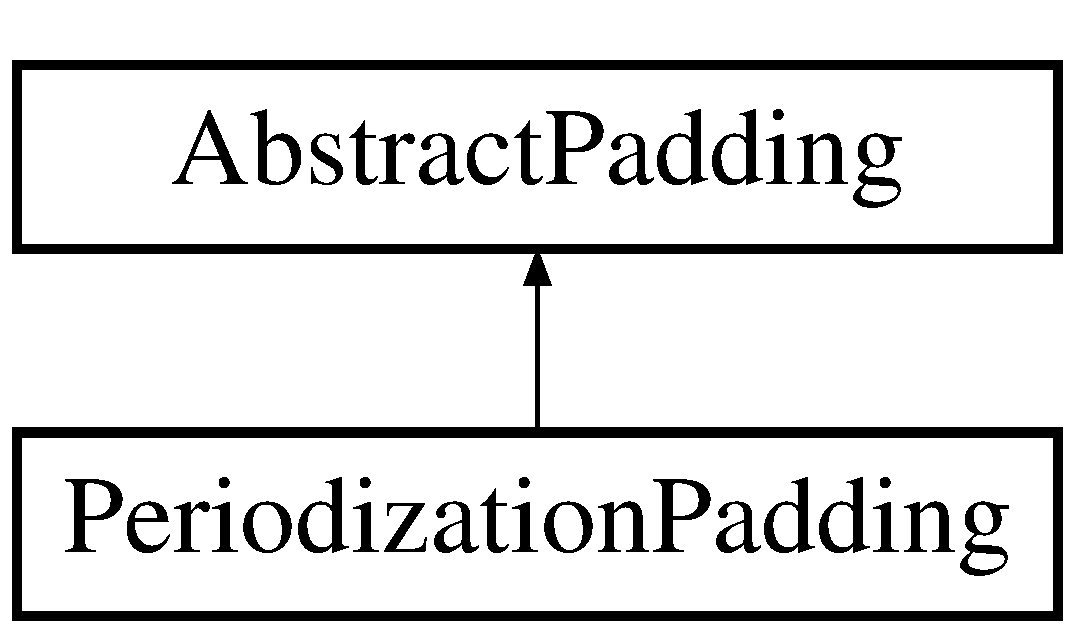
\includegraphics[height=2.000000cm]{class_periodization_padding}
\end{center}
\end{figure}
\subsection*{Public Member Functions}
\begin{DoxyCompactItemize}
\item 
\mbox{\Hypertarget{class_periodization_padding_a00b3d9784fa3319fe65dcc05b8353371}\label{class_periodization_padding_a00b3d9784fa3319fe65dcc05b8353371}} 
\hyperlink{class_image_pix}{Image\+Pix}$<$ int $>$ {\bfseries Perform\+Pad} (\hyperlink{class_image_pix}{Image\+Pix}$<$ int $>$ \&in)
\end{DoxyCompactItemize}


\subsection{Detailed Description}
Performs the Periodization of the image. 

The documentation for this class was generated from the following files\+:\begin{DoxyCompactItemize}
\item 
Periodization\+Padding.\+hpp\item 
Periodization\+Padding.\+cpp\end{DoxyCompactItemize}

\hypertarget{class_unpad}{}\section{Unpad Class Reference}
\label{class_unpad}\index{Unpad@{Unpad}}
Inheritance diagram for Unpad\+:\begin{figure}[H]
\begin{center}
\leavevmode
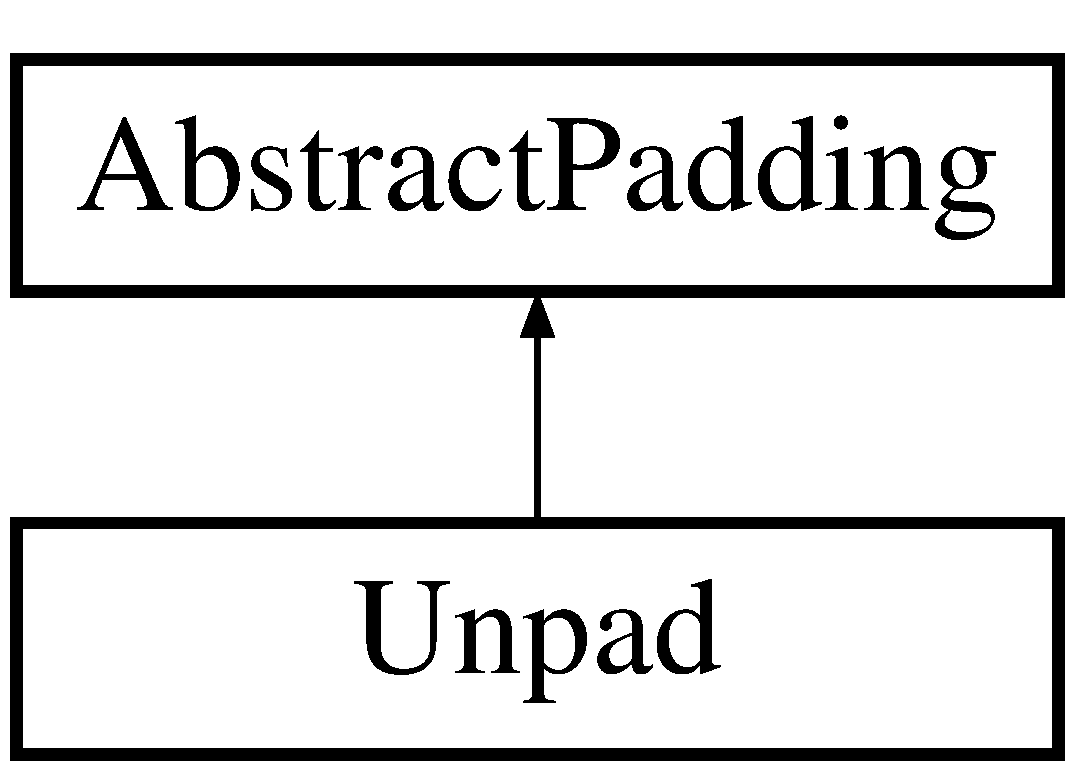
\includegraphics[height=2.000000cm]{class_unpad}
\end{center}
\end{figure}
\subsection*{Public Member Functions}
\begin{DoxyCompactItemize}
\item 
\mbox{\Hypertarget{class_unpad_aa32b832e71f6b6e69a9ba8e7965573da}\label{class_unpad_aa32b832e71f6b6e69a9ba8e7965573da}} 
\hyperlink{class_image_pix}{Image\+Pix}$<$ int $>$ {\bfseries Perform\+Pad} (\hyperlink{class_image_pix}{Image\+Pix}$<$ int $>$ \&in)
\item 
\mbox{\Hypertarget{class_unpad_ab38bc3289f7cedeccf4c56d918c48261}\label{class_unpad_ab38bc3289f7cedeccf4c56d918c48261}} 
\hyperlink{class_image_pix}{Image\+Pix}$<$ \hyperlink{class_complex_number}{Complex\+Number} $>$ {\bfseries Perform\+Pad\+Cplx} (\hyperlink{class_image_pix}{Image\+Pix}$<$ \hyperlink{class_complex_number}{Complex\+Number} $>$ \&in)
\end{DoxyCompactItemize}


The documentation for this class was generated from the following files\+:\begin{DoxyCompactItemize}
\item 
Unpad.\+hpp\item 
Unpad.\+cpp\end{DoxyCompactItemize}

\hypertarget{class_zero_padding}{}\section{Zero\+Padding Class Reference}
\label{class_zero_padding}\index{Zero\+Padding@{Zero\+Padding}}


{\ttfamily \#include $<$Zero\+Padding.\+hpp$>$}

Inheritance diagram for Zero\+Padding\+:\begin{figure}[H]
\begin{center}
\leavevmode
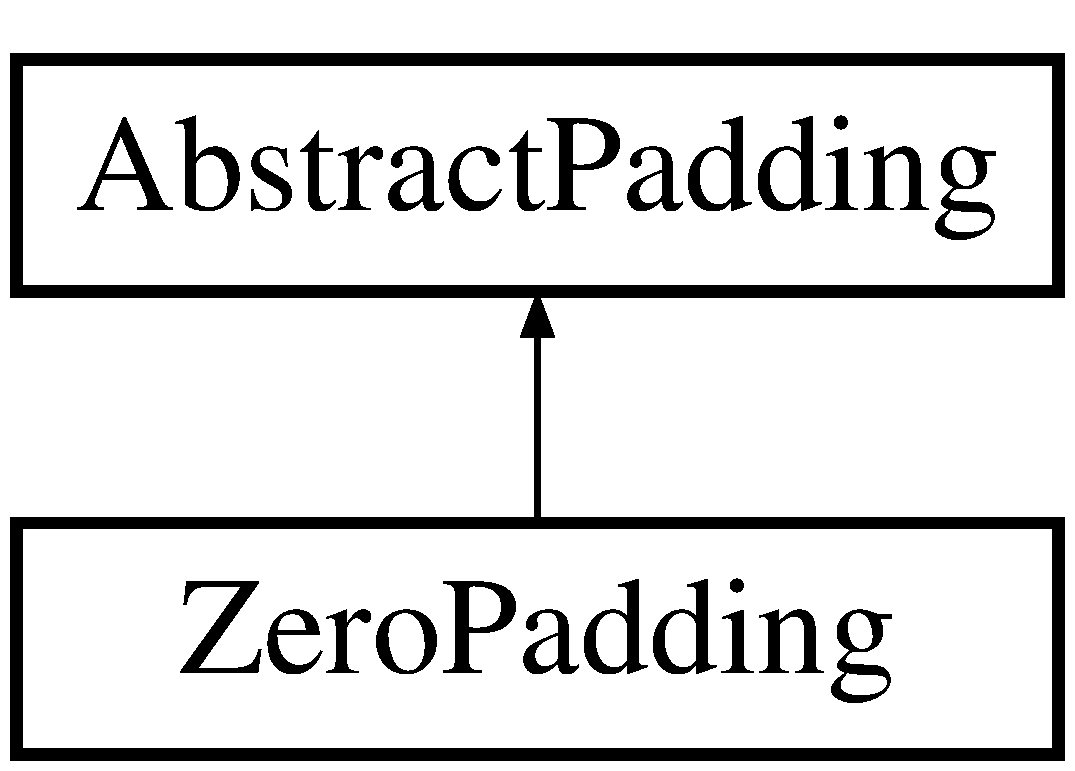
\includegraphics[height=2.000000cm]{class_zero_padding}
\end{center}
\end{figure}
\subsection*{Public Member Functions}
\begin{DoxyCompactItemize}
\item 
\mbox{\Hypertarget{class_zero_padding_af321474d0c1285317d38f01a7b91ed7d}\label{class_zero_padding_af321474d0c1285317d38f01a7b91ed7d}} 
\hyperlink{class_image_pix}{Image\+Pix}$<$ int $>$ {\bfseries Perform\+Pad} (\hyperlink{class_image_pix}{Image\+Pix}$<$ int $>$ \&in)
\end{DoxyCompactItemize}


\subsection{Detailed Description}
Performs the zero padding of the image. 

The documentation for this class was generated from the following files\+:\begin{DoxyCompactItemize}
\item 
Zero\+Padding.\+hpp\item 
Zero\+Padding.\+cpp\end{DoxyCompactItemize}

%--- End generated contents ---

% Index
\backmatter
\newpage
\phantomsection
\clearemptydoublepage
\addcontentsline{toc}{chapter}{Index}
\printindex

\end{document}
